% Options for packages loaded elsewhere
\PassOptionsToPackage{unicode}{hyperref}
\PassOptionsToPackage{hyphens}{url}
\PassOptionsToPackage{dvipsnames,svgnames,x11names}{xcolor}
%
\documentclass[
  11pt,
]{article}

\usepackage{amsmath,amssymb}
\usepackage{iftex}
\ifPDFTeX
  \usepackage[T1]{fontenc}
  \usepackage[utf8]{inputenc}
  \usepackage{textcomp} % provide euro and other symbols
\else % if luatex or xetex
  \usepackage{unicode-math}
  \defaultfontfeatures{Scale=MatchLowercase}
  \defaultfontfeatures[\rmfamily]{Ligatures=TeX,Scale=1}
\fi
\usepackage{lmodern}
\ifPDFTeX\else  
    % xetex/luatex font selection
\fi
% Use upquote if available, for straight quotes in verbatim environments
\IfFileExists{upquote.sty}{\usepackage{upquote}}{}
\IfFileExists{microtype.sty}{% use microtype if available
  \usepackage[]{microtype}
  \UseMicrotypeSet[protrusion]{basicmath} % disable protrusion for tt fonts
}{}
\makeatletter
\@ifundefined{KOMAClassName}{% if non-KOMA class
  \IfFileExists{parskip.sty}{%
    \usepackage{parskip}
  }{% else
    \setlength{\parindent}{0pt}
    \setlength{\parskip}{6pt plus 2pt minus 1pt}}
}{% if KOMA class
  \KOMAoptions{parskip=half}}
\makeatother
\usepackage{xcolor}
\usepackage[left=2.54cm,right=2.54cm]{geometry}
\setlength{\emergencystretch}{3em} % prevent overfull lines
\setcounter{secnumdepth}{-\maxdimen} % remove section numbering
% Make \paragraph and \subparagraph free-standing
\makeatletter
\ifx\paragraph\undefined\else
  \let\oldparagraph\paragraph
  \renewcommand{\paragraph}{
    \@ifstar
      \xxxParagraphStar
      \xxxParagraphNoStar
  }
  \newcommand{\xxxParagraphStar}[1]{\oldparagraph*{#1}\mbox{}}
  \newcommand{\xxxParagraphNoStar}[1]{\oldparagraph{#1}\mbox{}}
\fi
\ifx\subparagraph\undefined\else
  \let\oldsubparagraph\subparagraph
  \renewcommand{\subparagraph}{
    \@ifstar
      \xxxSubParagraphStar
      \xxxSubParagraphNoStar
  }
  \newcommand{\xxxSubParagraphStar}[1]{\oldsubparagraph*{#1}\mbox{}}
  \newcommand{\xxxSubParagraphNoStar}[1]{\oldsubparagraph{#1}\mbox{}}
\fi
\makeatother


\providecommand{\tightlist}{%
  \setlength{\itemsep}{0pt}\setlength{\parskip}{0pt}}\usepackage{longtable,booktabs,array}
\usepackage{calc} % for calculating minipage widths
% Correct order of tables after \paragraph or \subparagraph
\usepackage{etoolbox}
\makeatletter
\patchcmd\longtable{\par}{\if@noskipsec\mbox{}\fi\par}{}{}
\makeatother
% Allow footnotes in longtable head/foot
\IfFileExists{footnotehyper.sty}{\usepackage{footnotehyper}}{\usepackage{footnote}}
\makesavenoteenv{longtable}
\usepackage{graphicx}
\makeatletter
\newsavebox\pandoc@box
\newcommand*\pandocbounded[1]{% scales image to fit in text height/width
  \sbox\pandoc@box{#1}%
  \Gscale@div\@tempa{\textheight}{\dimexpr\ht\pandoc@box+\dp\pandoc@box\relax}%
  \Gscale@div\@tempb{\linewidth}{\wd\pandoc@box}%
  \ifdim\@tempb\p@<\@tempa\p@\let\@tempa\@tempb\fi% select the smaller of both
  \ifdim\@tempa\p@<\p@\scalebox{\@tempa}{\usebox\pandoc@box}%
  \else\usebox{\pandoc@box}%
  \fi%
}
% Set default figure placement to htbp
\def\fps@figure{htbp}
\makeatother

\usepackage[noblocks]{authblk}
\renewcommand*{\Authsep}{, }
\renewcommand*{\Authand}{, }
\renewcommand*{\Authands}{, }
\renewcommand\Affilfont{\small}
\usepackage{lipsum} \usepackage{libertine}
\makeatletter
\@ifpackageloaded{caption}{}{\usepackage{caption}}
\AtBeginDocument{%
\ifdefined\contentsname
  \renewcommand*\contentsname{Table of contents}
\else
  \newcommand\contentsname{Table of contents}
\fi
\ifdefined\listfigurename
  \renewcommand*\listfigurename{List of Figures}
\else
  \newcommand\listfigurename{List of Figures}
\fi
\ifdefined\listtablename
  \renewcommand*\listtablename{List of Tables}
\else
  \newcommand\listtablename{List of Tables}
\fi
\ifdefined\figurename
  \renewcommand*\figurename{Figure}
\else
  \newcommand\figurename{Figure}
\fi
\ifdefined\tablename
  \renewcommand*\tablename{Table}
\else
  \newcommand\tablename{Table}
\fi
}
\@ifpackageloaded{float}{}{\usepackage{float}}
\floatstyle{ruled}
\@ifundefined{c@chapter}{\newfloat{codelisting}{h}{lop}}{\newfloat{codelisting}{h}{lop}[chapter]}
\floatname{codelisting}{Listing}
\newcommand*\listoflistings{\listof{codelisting}{List of Listings}}
\makeatother
\makeatletter
\makeatother
\makeatletter
\@ifpackageloaded{caption}{}{\usepackage{caption}}
\@ifpackageloaded{subcaption}{}{\usepackage{subcaption}}
\makeatother

\usepackage{bookmark}

\IfFileExists{xurl.sty}{\usepackage{xurl}}{} % add URL line breaks if available
\urlstyle{same} % disable monospaced font for URLs
\hypersetup{
  pdftitle={Supplementary Material: Producing population-level estimates of internal displacement in Ukraine using GPS mobile phone data},
  pdfauthor={Anonymised for peer review},
  colorlinks=true,
  linkcolor={blue},
  filecolor={Maroon},
  citecolor={Blue},
  urlcolor={Blue},
  pdfcreator={LaTeX via pandoc}}


\title{\textbf{Supplementary Material: Producing population-level
estimates of internal displacement in Ukraine using GPS mobile phone
data}}


\author{Anonymised for peer review}



\date{}
\begin{document}
\maketitle


\newpage

\section{Supplementary Tables}\label{supplementary-tables}

\textbf{Supplementary Table 1: National-level estimates of internal
population displacement, February to August 2024.} We assess the
accuracy of our estimates of population displacement against published
estimates produced by (1) IOM (International Organization for Migration)
in the fourth column, and (2) Leasure and team in the fifth column. As
described in the manuscript, IOM estimates are based on a telephone
survey of 2,000 individuals each month. Leasure et al's estimates are
based on data from Facebook's Advertising Platform. Unlike these
efforts, and as described in the Methods section, our estimates are
based on GPS mobile phone data. For our comparative assessment in this
section, we report national estimates including and excluding Crimea. We
use the former for our main analysis in the manuscript, and use the
latter for our analysis here as these estimates are the most comparable
to those produced by the IOM and Leasure et al which do not consider the
Crimea oblast and Russian-occupied areas prior to the 2022 invasion. Our
national-level estimates display a relatively high degree of
correspondence with IOM estimates, particularly from March to July, and
they tend to be higher than those produced by Leasure et al.~by
approximately 250 thousand people across the time series. The difference
with estimates produced by Leasure and team may be explained by the fact
that they are affected by power outages in the Donetsk and Luhansk
regions, resulting in no or very small estimates for various dates after
March 2022 and multiple locations. Supplementary Figures 2-4 capture
this absence of estimates.

\phantomsection\label{tab-national}
\begin{center}
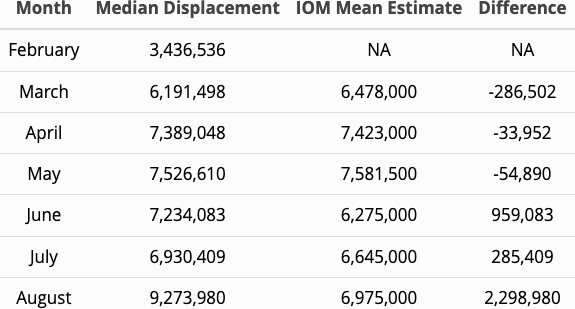
\includegraphics[width=0.6\linewidth,height=\textheight,keepaspectratio]{../outputs/sm/tables/table_all_estimates.png}
\end{center}

\newpage

\section{Supplementary Figures}\label{supplementary-figures}

\textbf{Supplementary Figure 1: Distribution of distance travelled
relating to internal population movements.} We analyse the distribution
of distance travelled, computing the Haversine distance in kilometres
based on centriods between areas at the raion level. We compute the
distance for all moves, involving the home location as a starting point,
temporary locations and the ``final'' destination area (i.e.~where
people spent most time away from their residential area). The results
indicate that most people travelled less than 100 kilometres and most
moves involves a displacement away from the home location. These results
suggest that most people move do not move that far from their home
location. While this is a common observed pattern for intentional moves,
it is less expected for forced displacements. The distance profile for
all moves is similar to that of return movements (Fig.3 reported in the
manuscript). This suggests that most displacements are made to their
``final'' semi-permanent destinations.

\begin{figure}[h]

\begin{minipage}{\linewidth}

\begin{center}
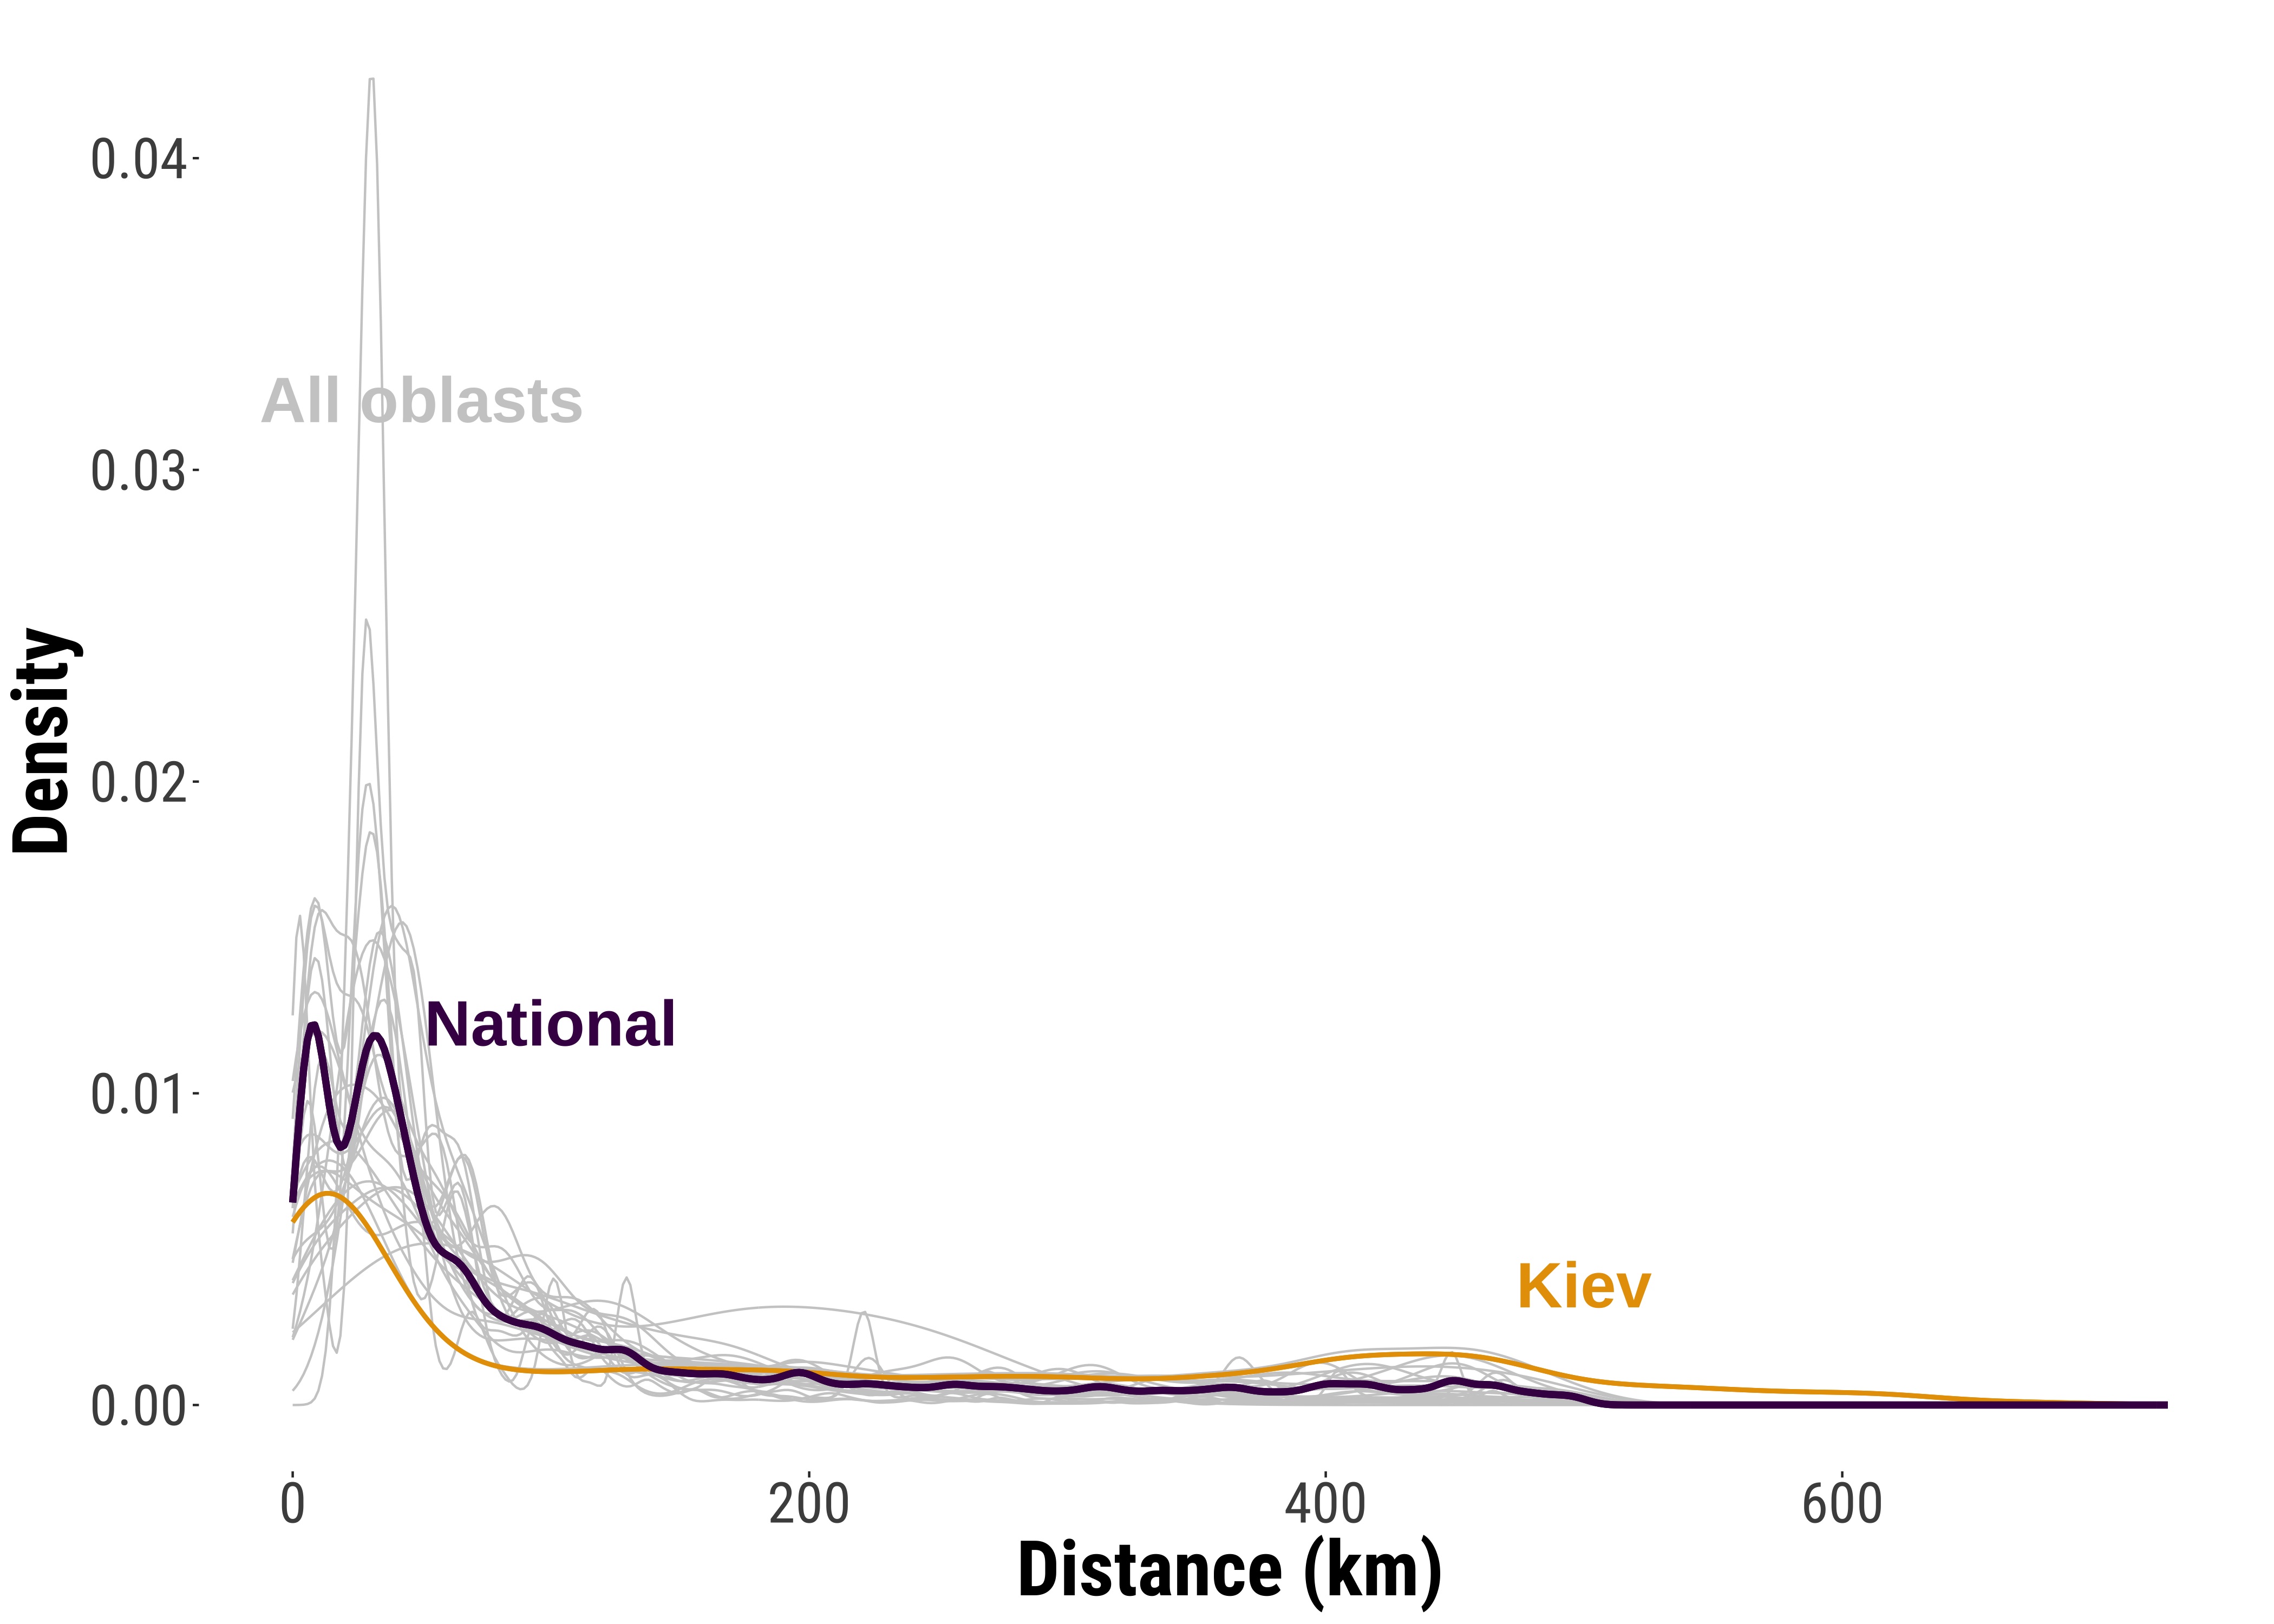
\includegraphics[width=5.20833in,height=\textheight,keepaspectratio]{../outputs/sm/distance_all-moves.png}
\end{center}

\end{minipage}%

\end{figure}%

\newpage

\textbf{Supplementary Figure 2: Correlation of coefficients based on
based on three data sources: GPS, IOM and FB estimates, Pearson and
Spearman, national regional and oblast level estimates.} We measure the
overall correlation between our GPS estimates and those derived by IOM
and Leasure and team from FB data. We compute Pearson and Spearman
correlation coefficients for estimates at three geographical levels:
national, regional and oblast levels. Again, we cannot evaluate our
estimates at the raion level as no comparable estimates for the period
of analysis were published for our assessment. The results reveal a high
degree of correspondence between our estimates and those produced by IOM
and Leasure and colleagues across Pearson and Spearman correlations
across the three levels of geography in our analysis.

\begin{figure}[h]

\begin{minipage}{\linewidth}

\pandocbounded{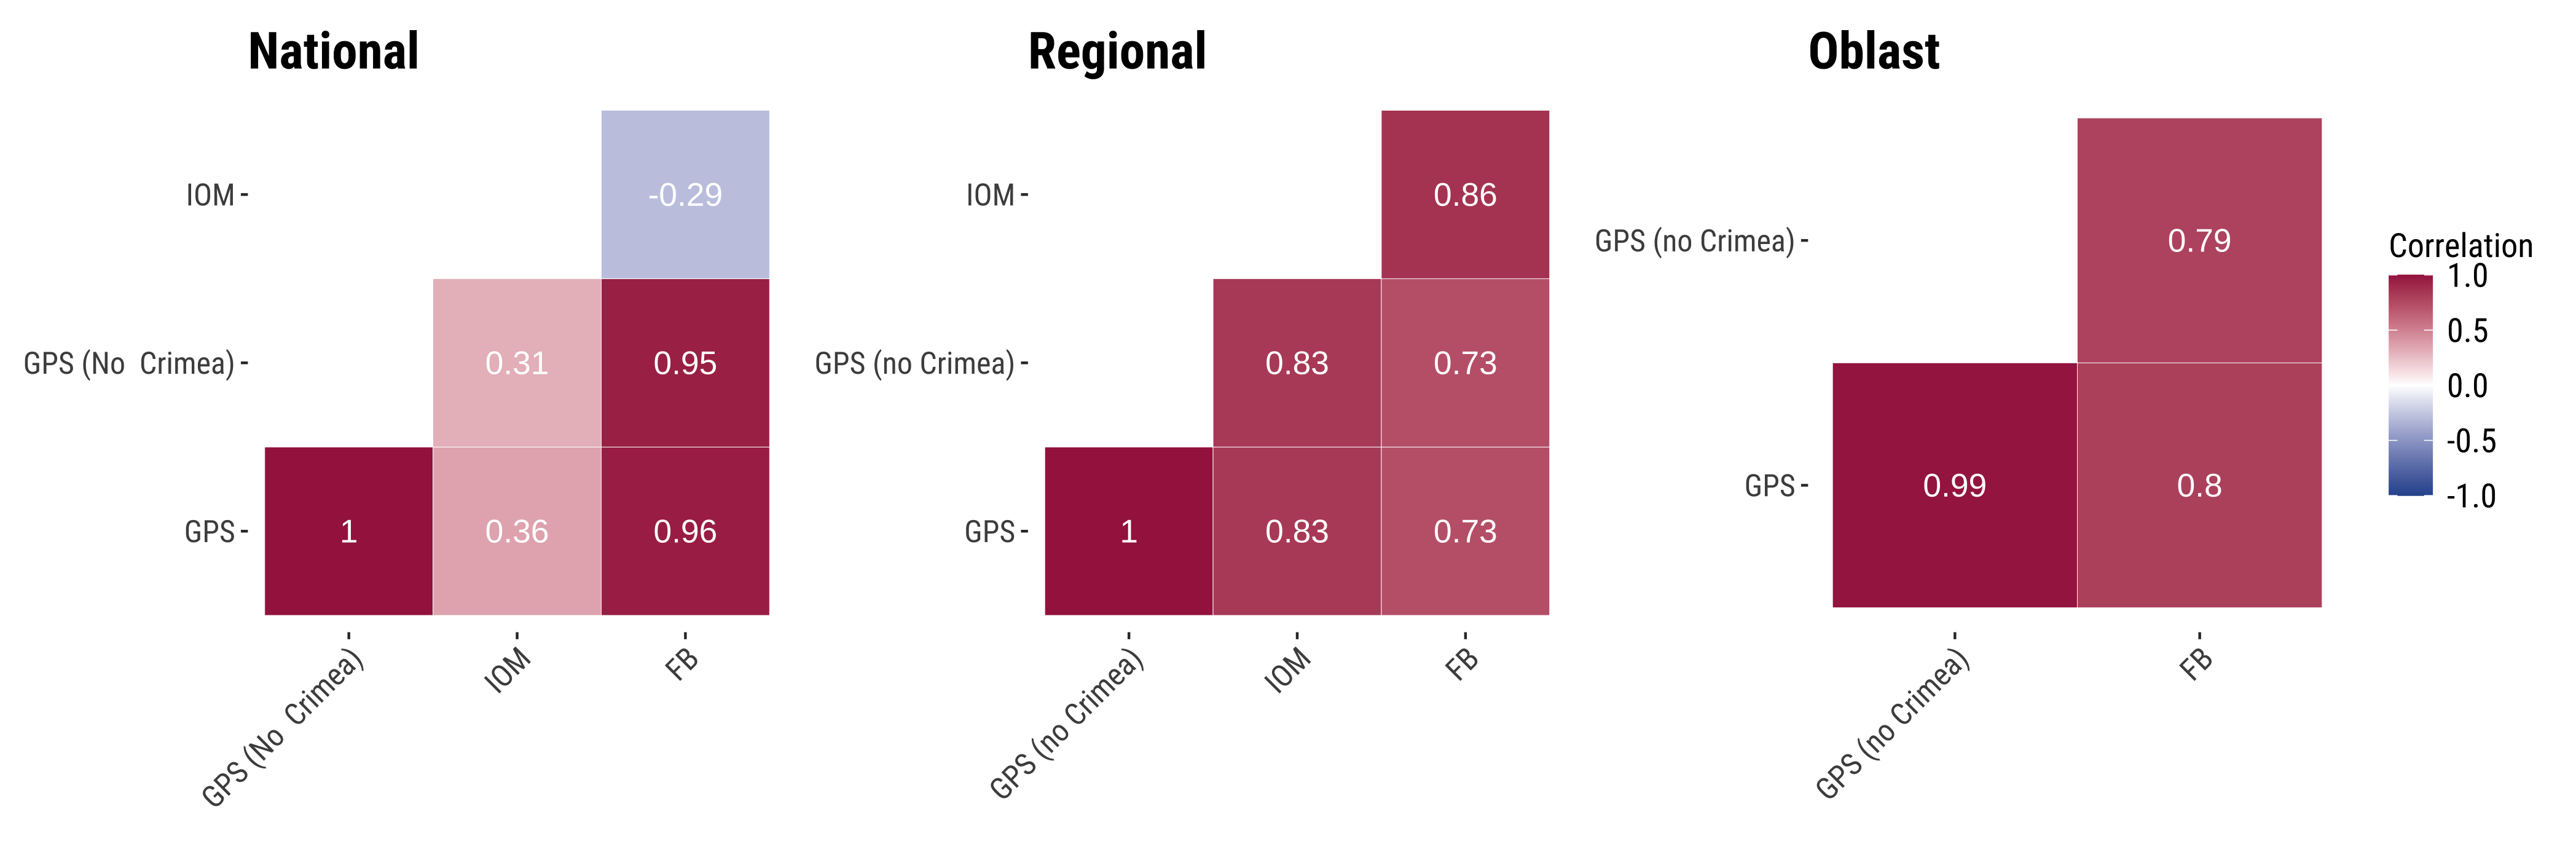
\includegraphics[keepaspectratio]{../outputs/sm/correlations_pearson.png}}

\subcaption{\label{}Pearson's correlations}
\end{minipage}%
\newline
\begin{minipage}{\linewidth}

\pandocbounded{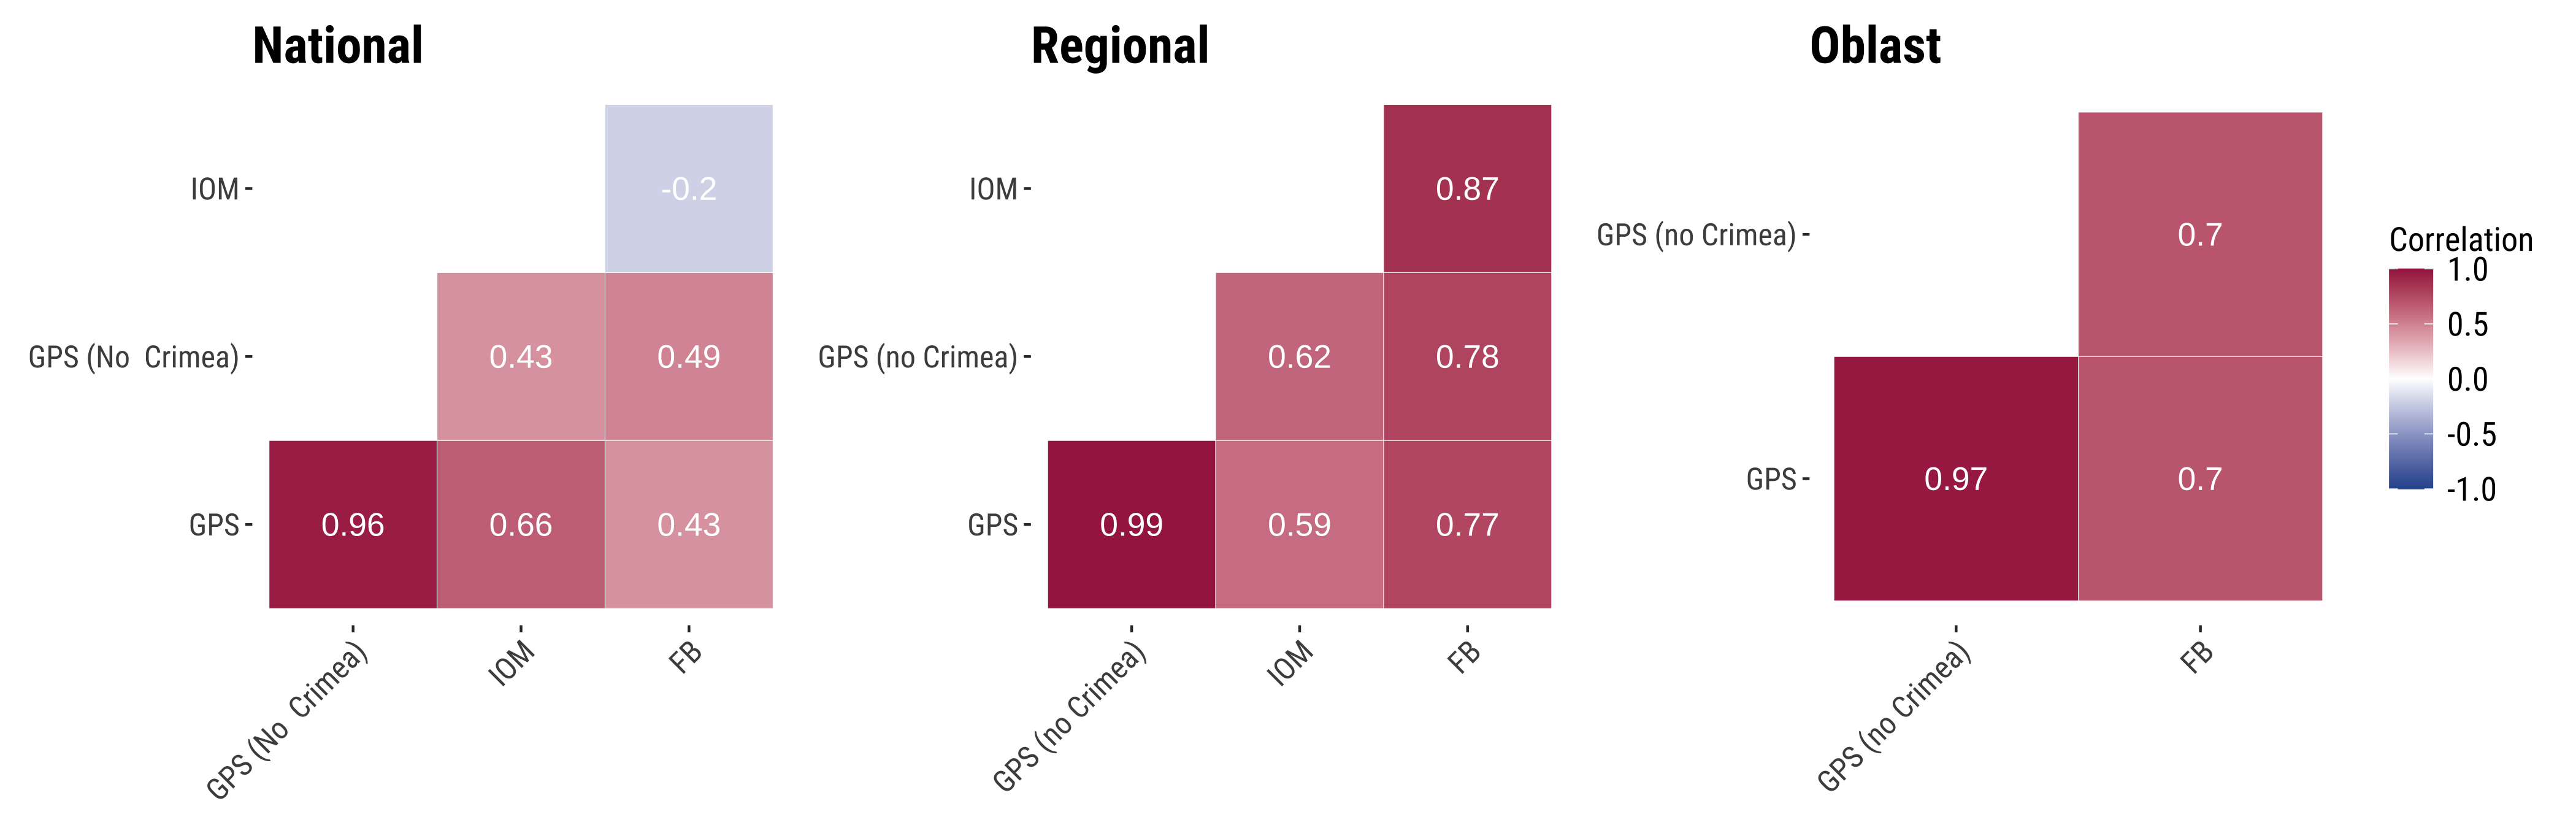
\includegraphics[keepaspectratio]{../outputs/sm/correlations_spearman.png}}

\subcaption{\label{}Spearman's correlations}
\end{minipage}%

\end{figure}%

\newpage

\textbf{Supplementary Figure 3: Regional-level estimates of internal
population displacement, based on three data sources: GPS, IOM and FB
estimates, February to August 2022.} We compare our GSP-based estimates
against the survey-based IOM and FB-based Leasure et al estimates for
macro-regional areas. We assess two dimensions of these estimates: (1)
their level, and (2) temporal. We expect them to display a similar scale
and temporal trend of displacement. As expected, all three sets of
estimates are largely consistent with small discrepancies. The most
notably systematic difference is against the FB-based estimates for the
East region. As explained in the manuscript, this reflects the fact that
Leasure et al.'s estimates are affected by power outages in the eastern
regions of Donetsk and Luhansk resulting in zero or small population
counts for the period of analysis. Additionally, our GPS-based estimates
display a larger number of population displacement for western areas,
capturing return movements from these regions to Kiev and northern
regions as Russian troops withdrew from these areas. We note that
FB-based estimates are only available until July so discrepancies
between our GPS-based estimates and those based on FB data are not
observable, and the identified differences for July and August are
specific to our and IOM's estimates.

\begin{figure}[h]

\begin{minipage}{\linewidth}

\begin{center}
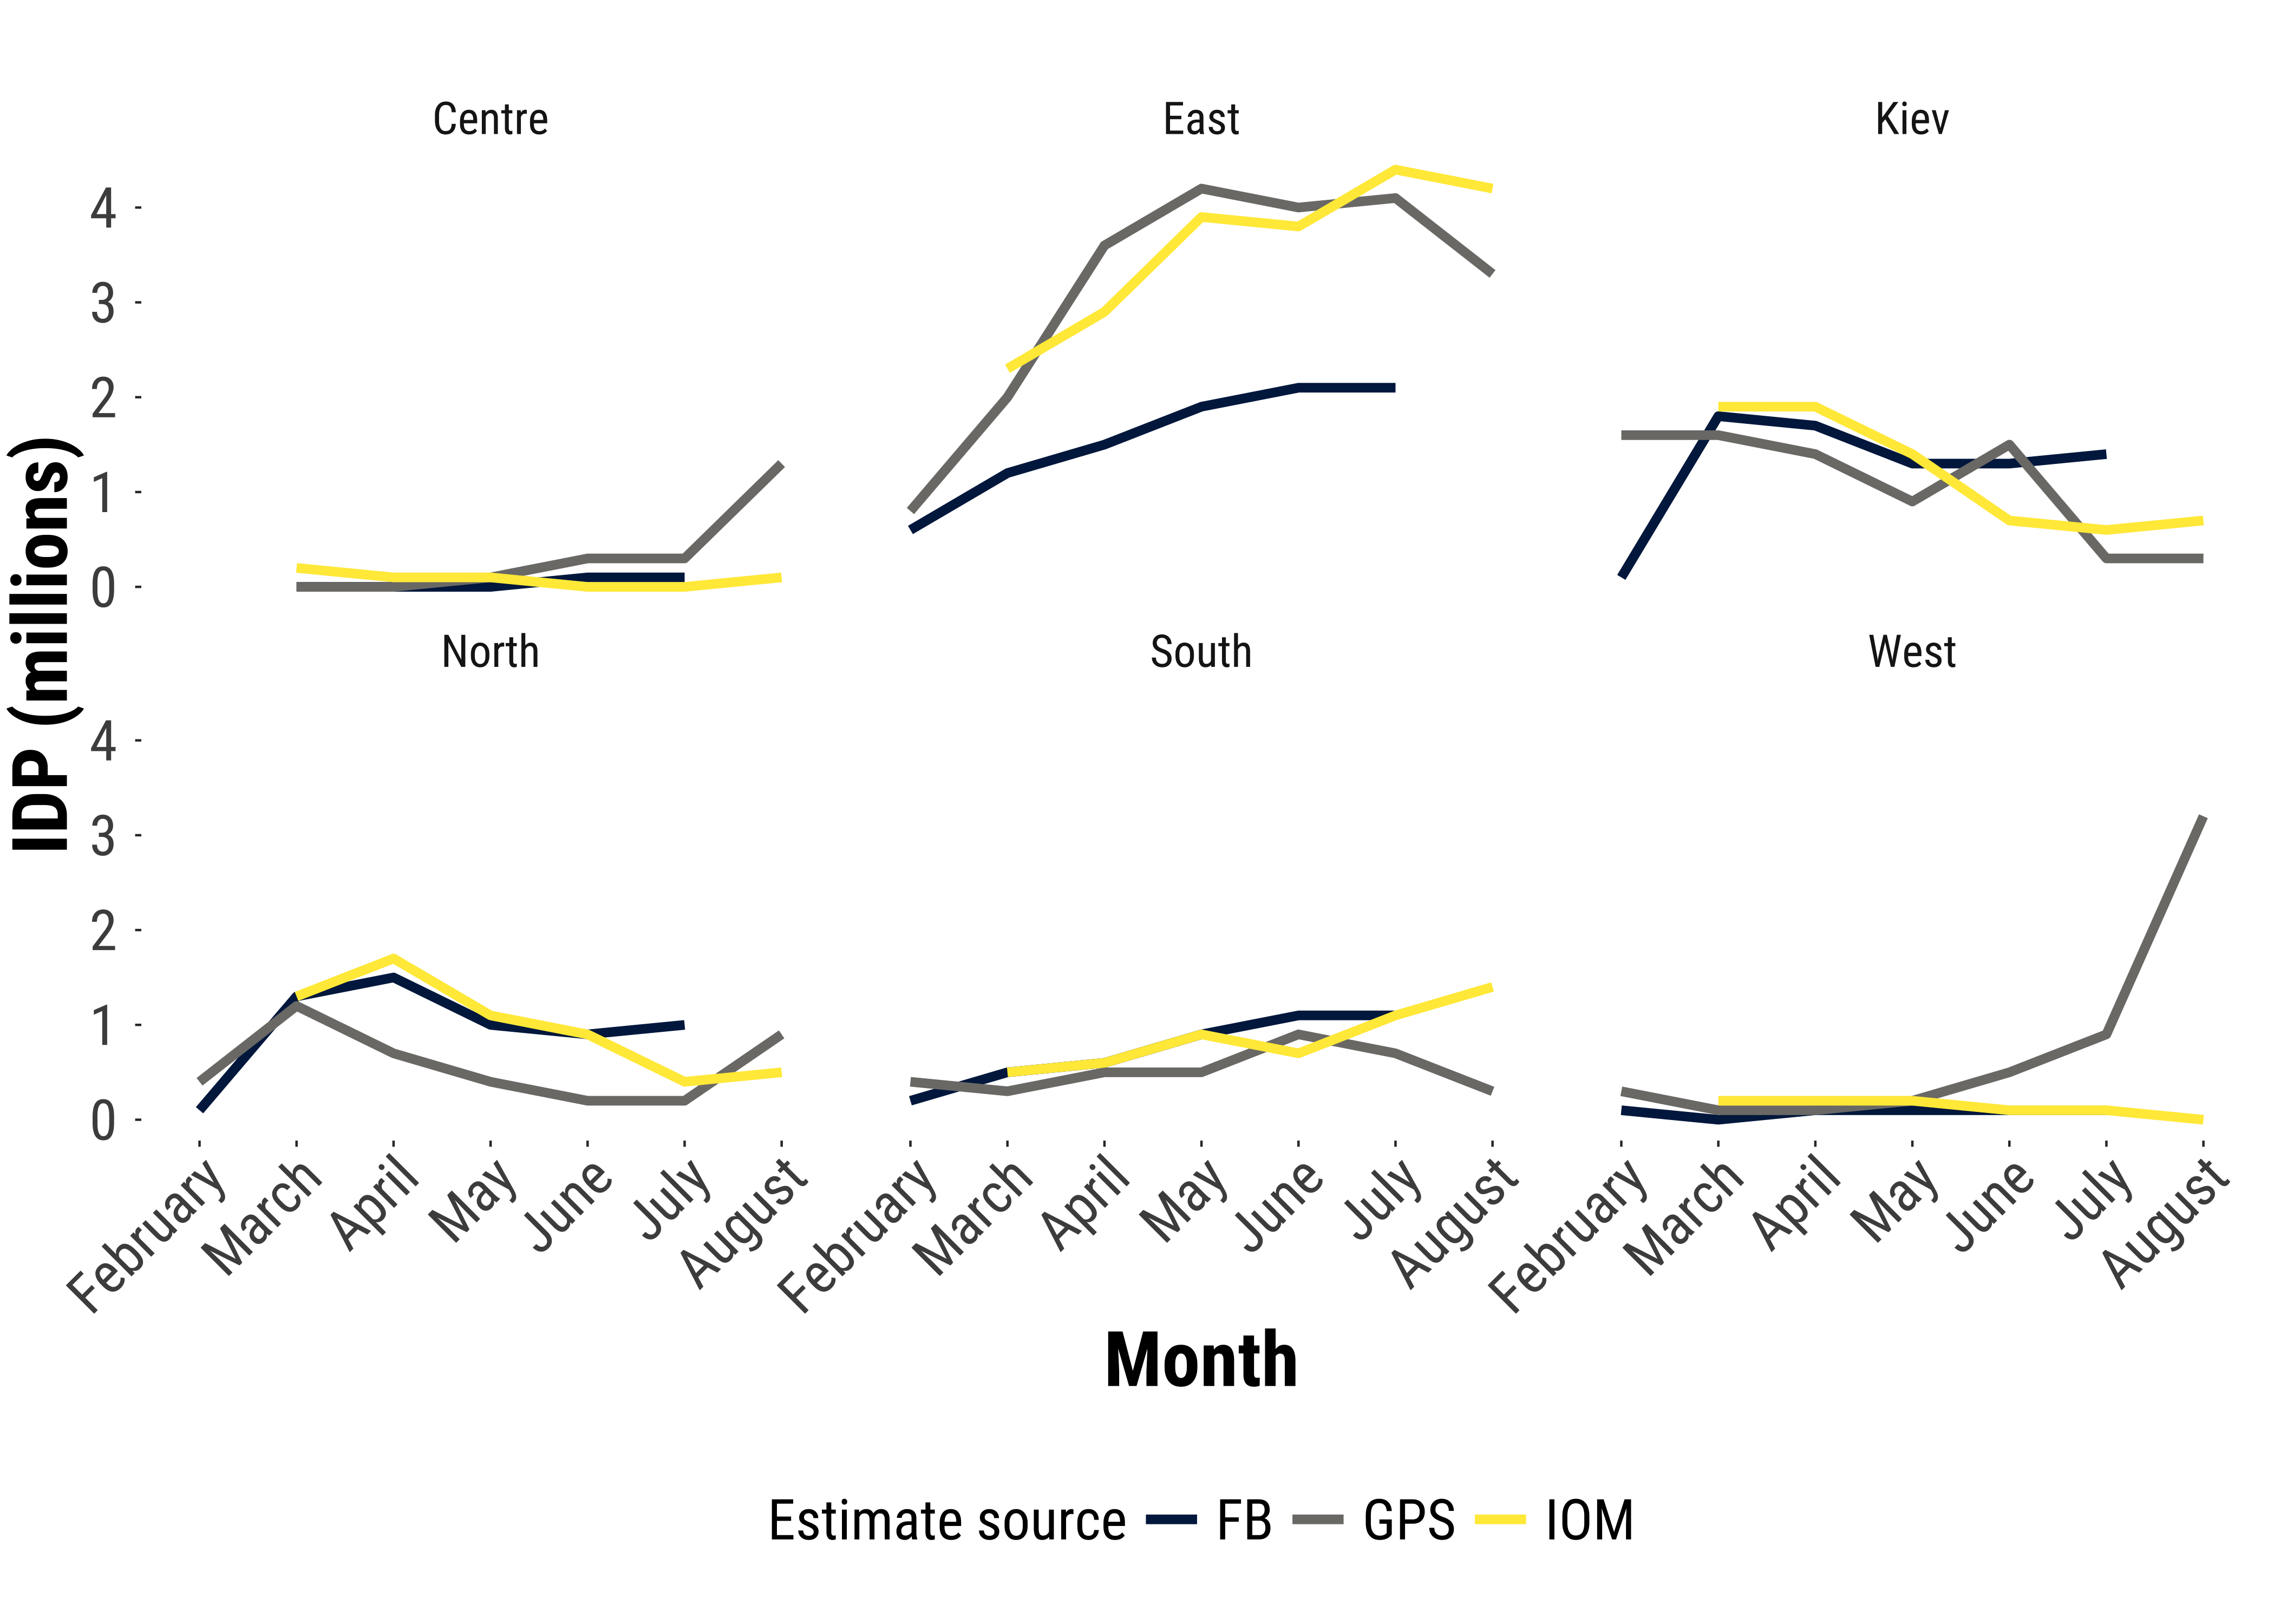
\includegraphics[width=5.20833in,height=\textheight,keepaspectratio]{../outputs/sm/plot_macro_region.png}
\end{center}

\end{minipage}%

\end{figure}%

\newpage

\textbf{Supplementary Figure 4: Oblasts-level estimates of internal
population displacement, based on two data sources: GPS and FB
estimates, February to August 2022.} We also compare our GSP-based
estimates against the FB-based Leasure et al estimates at the oblast
level. IOM have no published oblast-level estimates for the period of
analysis. Oblast comprises the most detailed geography at which internal
population displacement are published for the period of analysis. We
acknowledge that the IOM have started producing raion-level estimates
more recently but they are not openly accessible. As above, we assess
two dimensions: (1) the level, and (2) temporal alignment of the set of
estimates. Our GPS-based and the FB-based estimates show a remarkable
degree of correspondence. We note that FB-based estimates are not
available for some oblasts and time periods as a result of power
outages.

\begin{figure}[h]

\begin{minipage}{\linewidth}

\pandocbounded{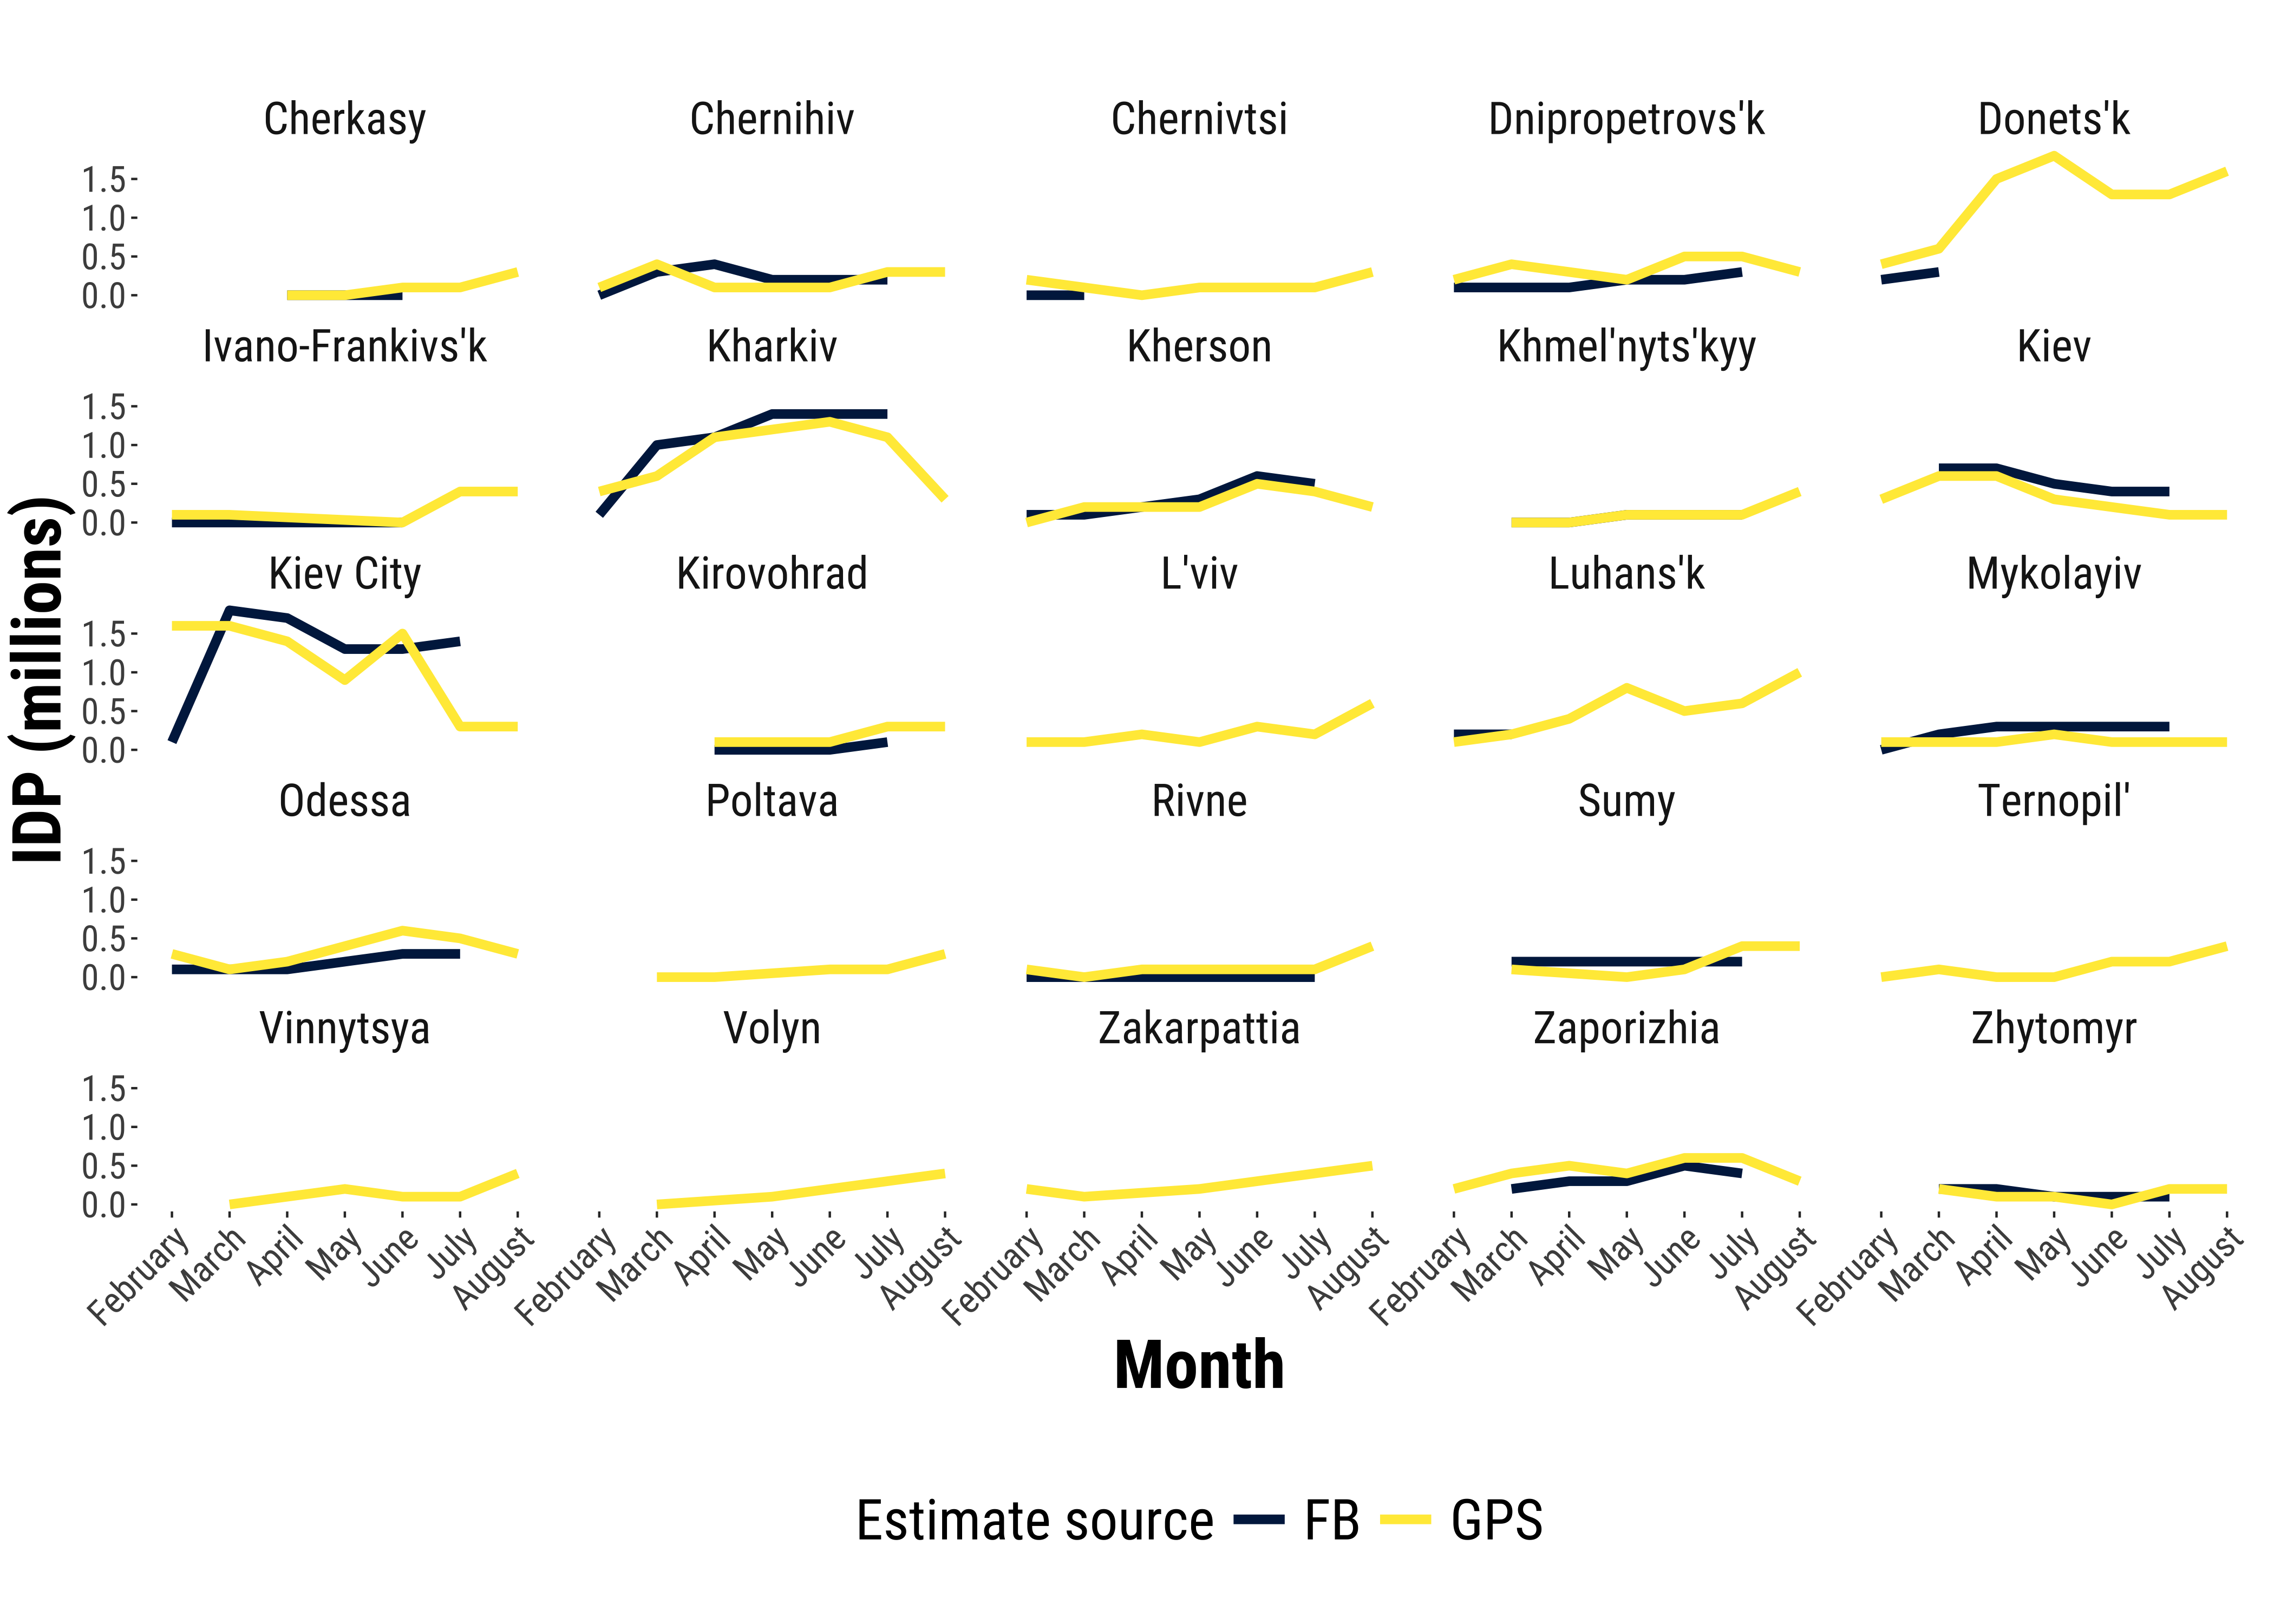
\includegraphics[keepaspectratio]{../outputs/sm/plot_oblast.png}}

\end{minipage}%

\end{figure}%

\newpage

\textbf{Supplementary Figure 5: National-level estimates of return
movement using two methods.} As described in the Methods Section, we
compare two approaches approaches to estimate the number of return
movement. These approaches are based on the methods used by: (1) the
IOM; and, (2) Leasure and team. We compare both sets of estimates and
considered that the latter approach provides more reasonable estimates:
1) the IOM approach generates estimates suggesting a decline in the
number of returns from over 2 million to around 500 thousand; 2) it
produces return estimates displaying an increasing trend, within the
range of 1 million in February 2022 and 4 million July 2022; and, 3)
Leasure el at approach produces estimates indicating an increasing trend
of return moves over time. The latter is what we expect based on
existing information, anecdotal evidence and news reporting. At the same
time, we consider a decline in the number of the number of IDP to be
unrealistic. As Russian troops withdrew from northern Ukraine, we have
visual and information evidence to suggest that many people returned to
Kiev and northern areas in June and July 2022. Additionally, the IOM
estimates uses a two-week period to define returns; that is, a returnee
is an individual who have left and return to their home location after a
two-week period. Our definition indicates that the mean duration time of
return moves is nine weeks.

\begin{figure}[h]

\begin{minipage}{0.50\linewidth}

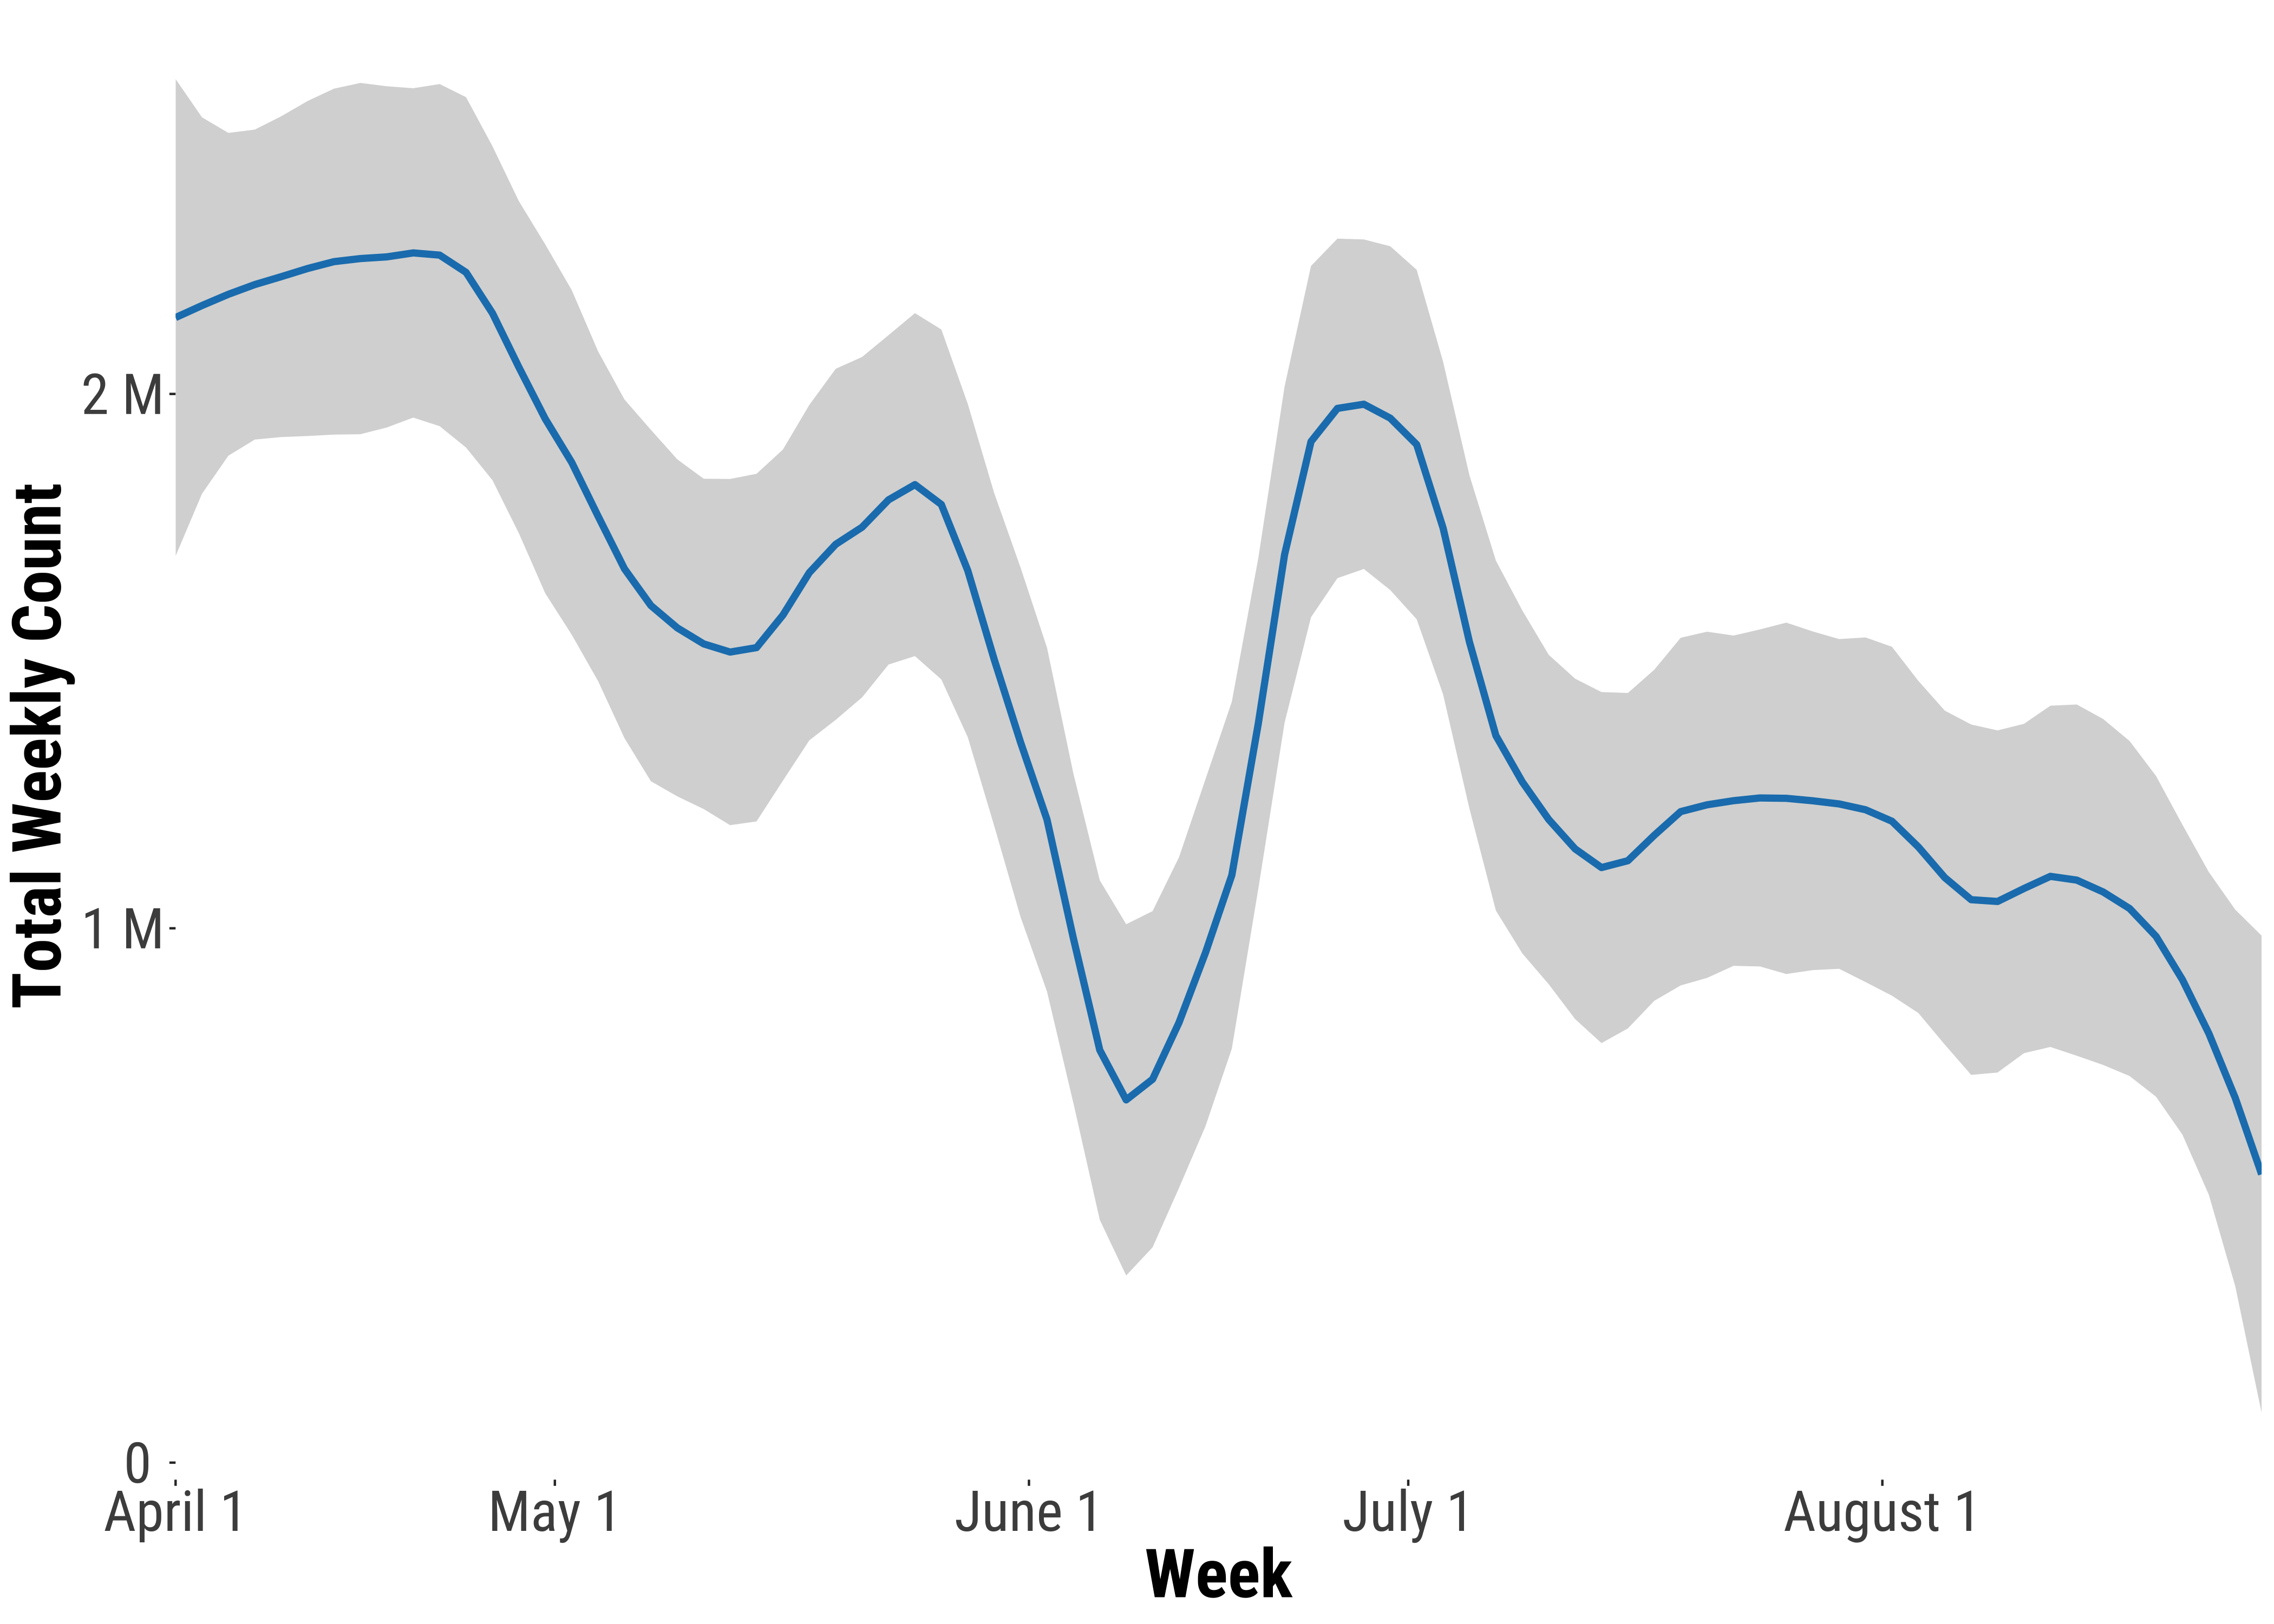
\includegraphics[width=3.02083in,height=\textheight,keepaspectratio]{../outputs/sm/ukr_wide_returns_iom.png}

\subcaption{\label{}IOM-based approach}
\end{minipage}%
%
\begin{minipage}{0.50\linewidth}

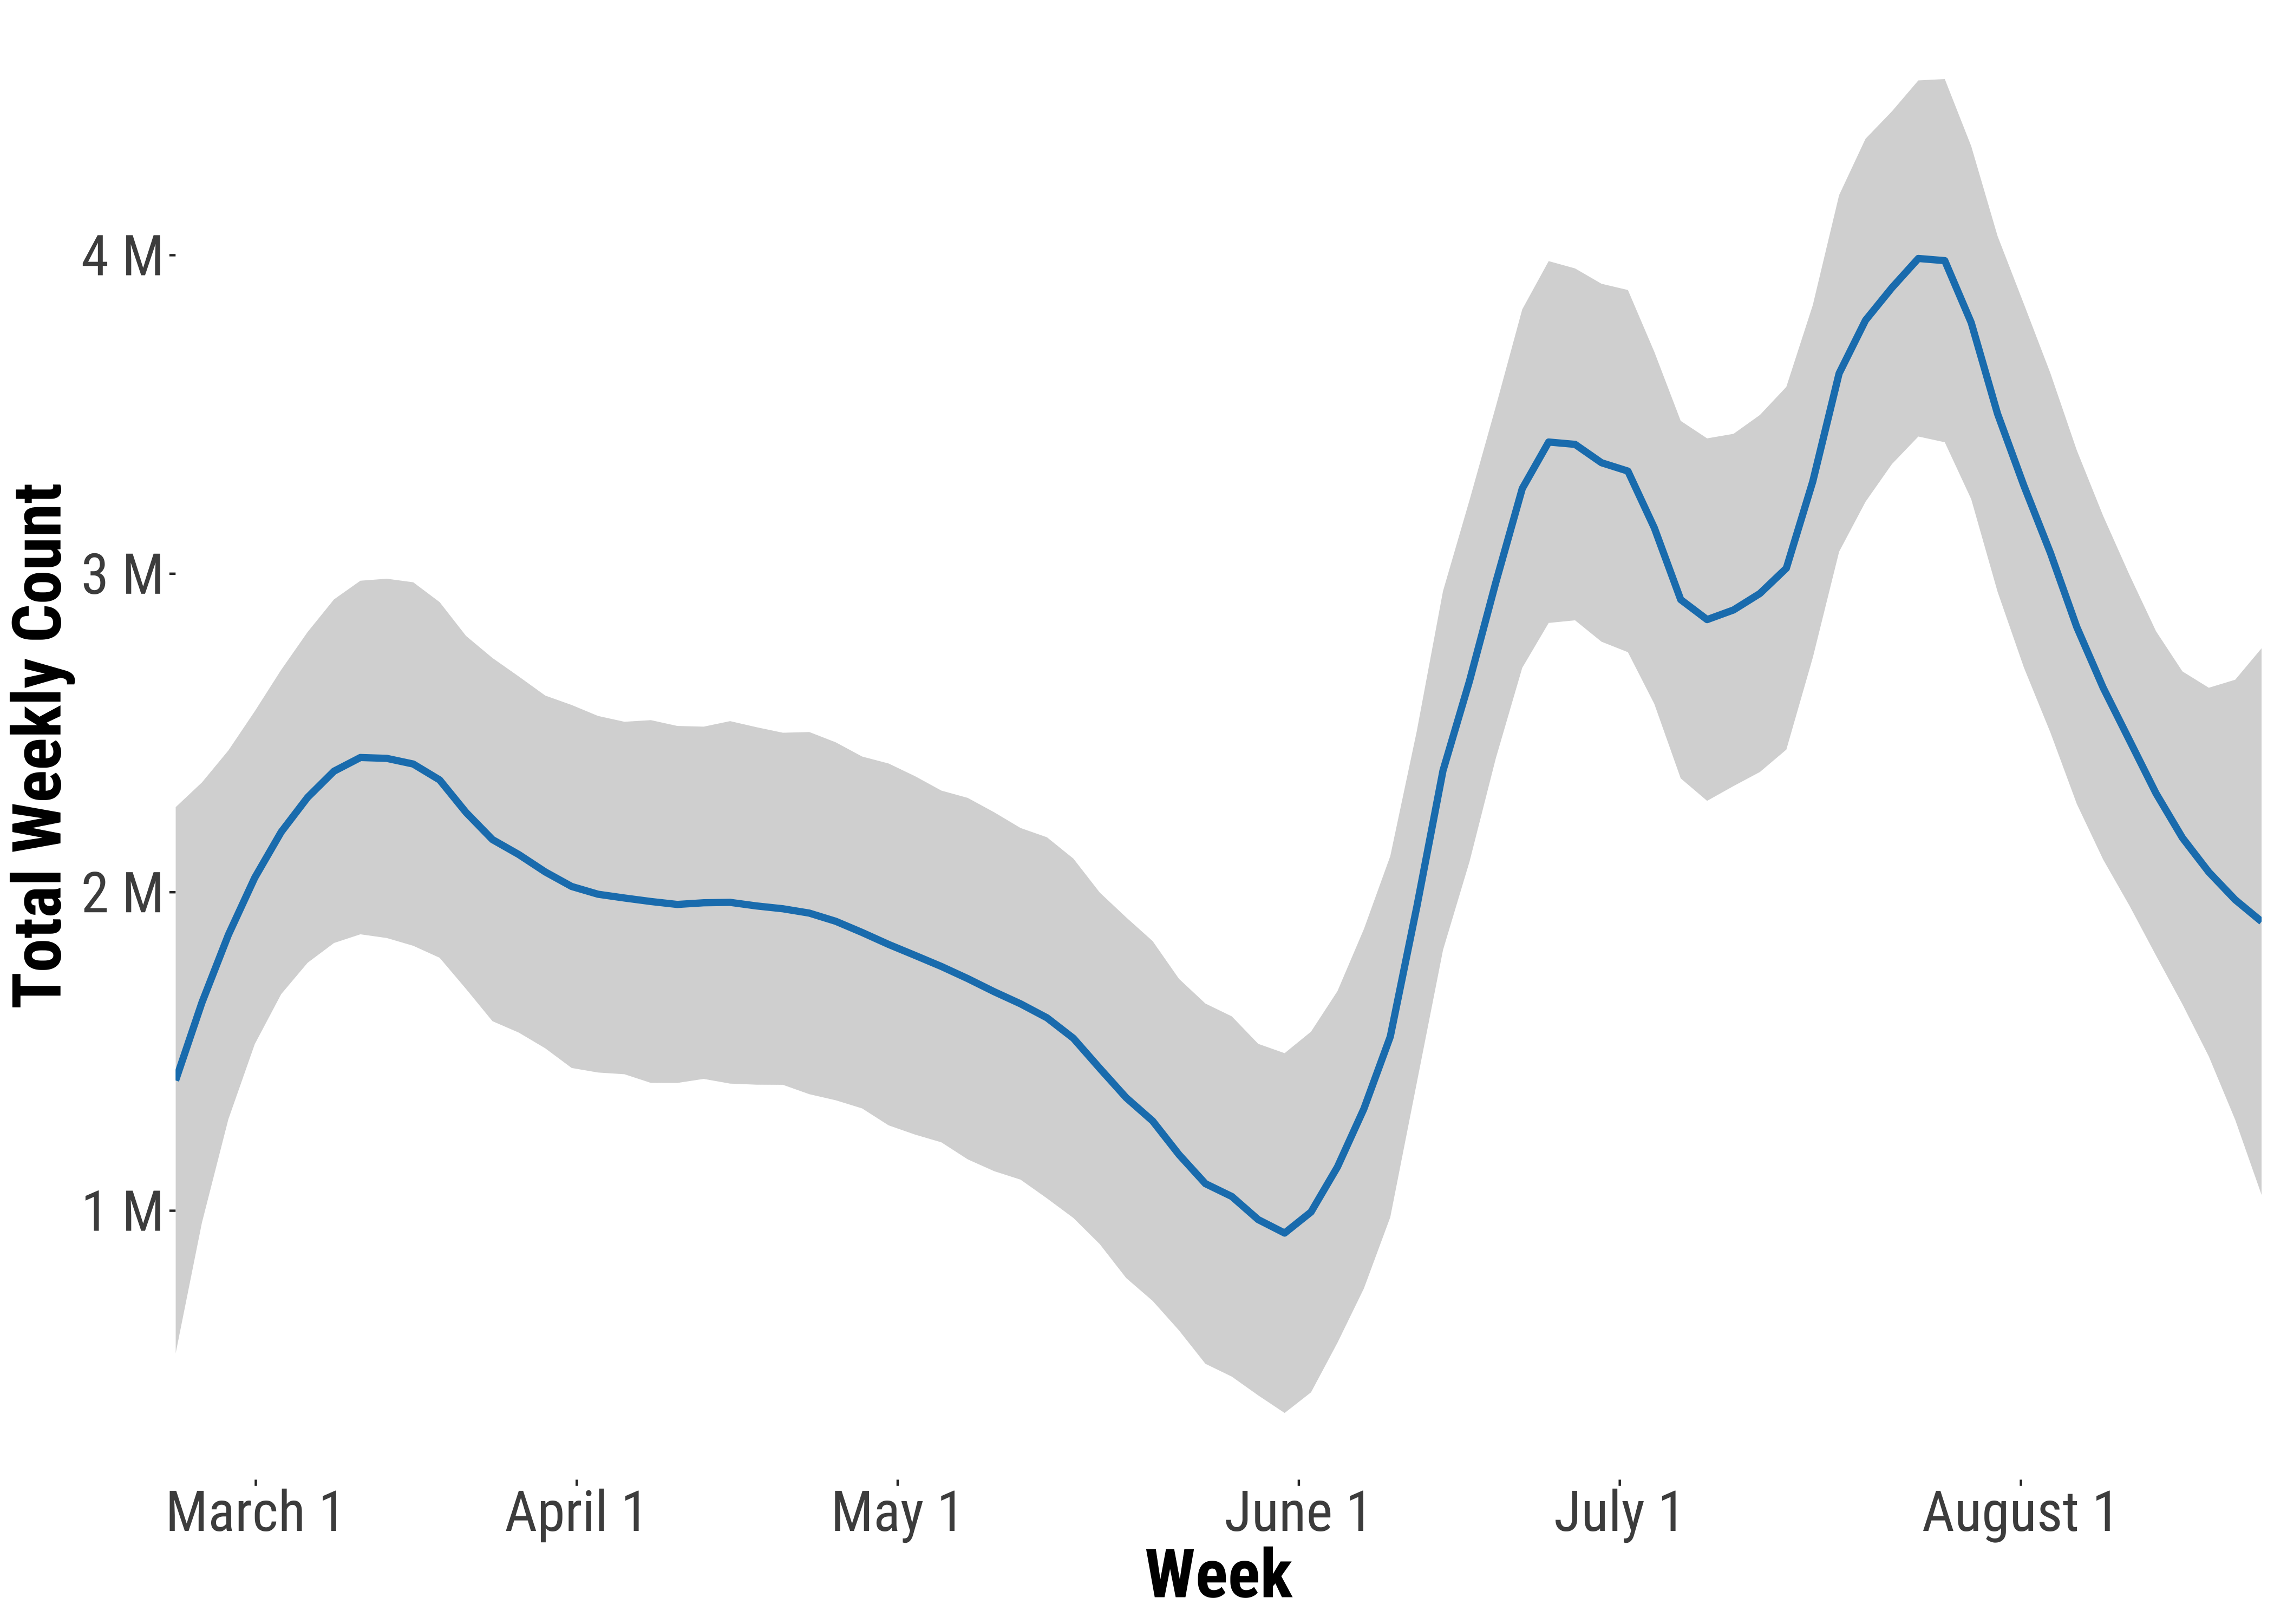
\includegraphics[width=3.02083in,height=\textheight,keepaspectratio]{../outputs/sm/ukr_wide_returns2_doug.png}

\subcaption{\label{}Leasure et al-based approach}
\end{minipage}%

\end{figure}%

\newpage

\textbf{Supplementary Figure 6: Number of weeks spent away from the
place of residence before returning.} We examine the distribution of
weeks before a return move to a home location occurred. The IOM
definition defines that a return occurs after people have spent two
weeks away from their home location. Our evidence indicates that the
average number of weeks before a return is observed is nine weeks after
people moved away from home. A very small percentage of people (less
than 3\%) appears to make a return to their home location after two
weeks away from home.

\begin{figure}

\begin{minipage}{\linewidth}
\begin{center}
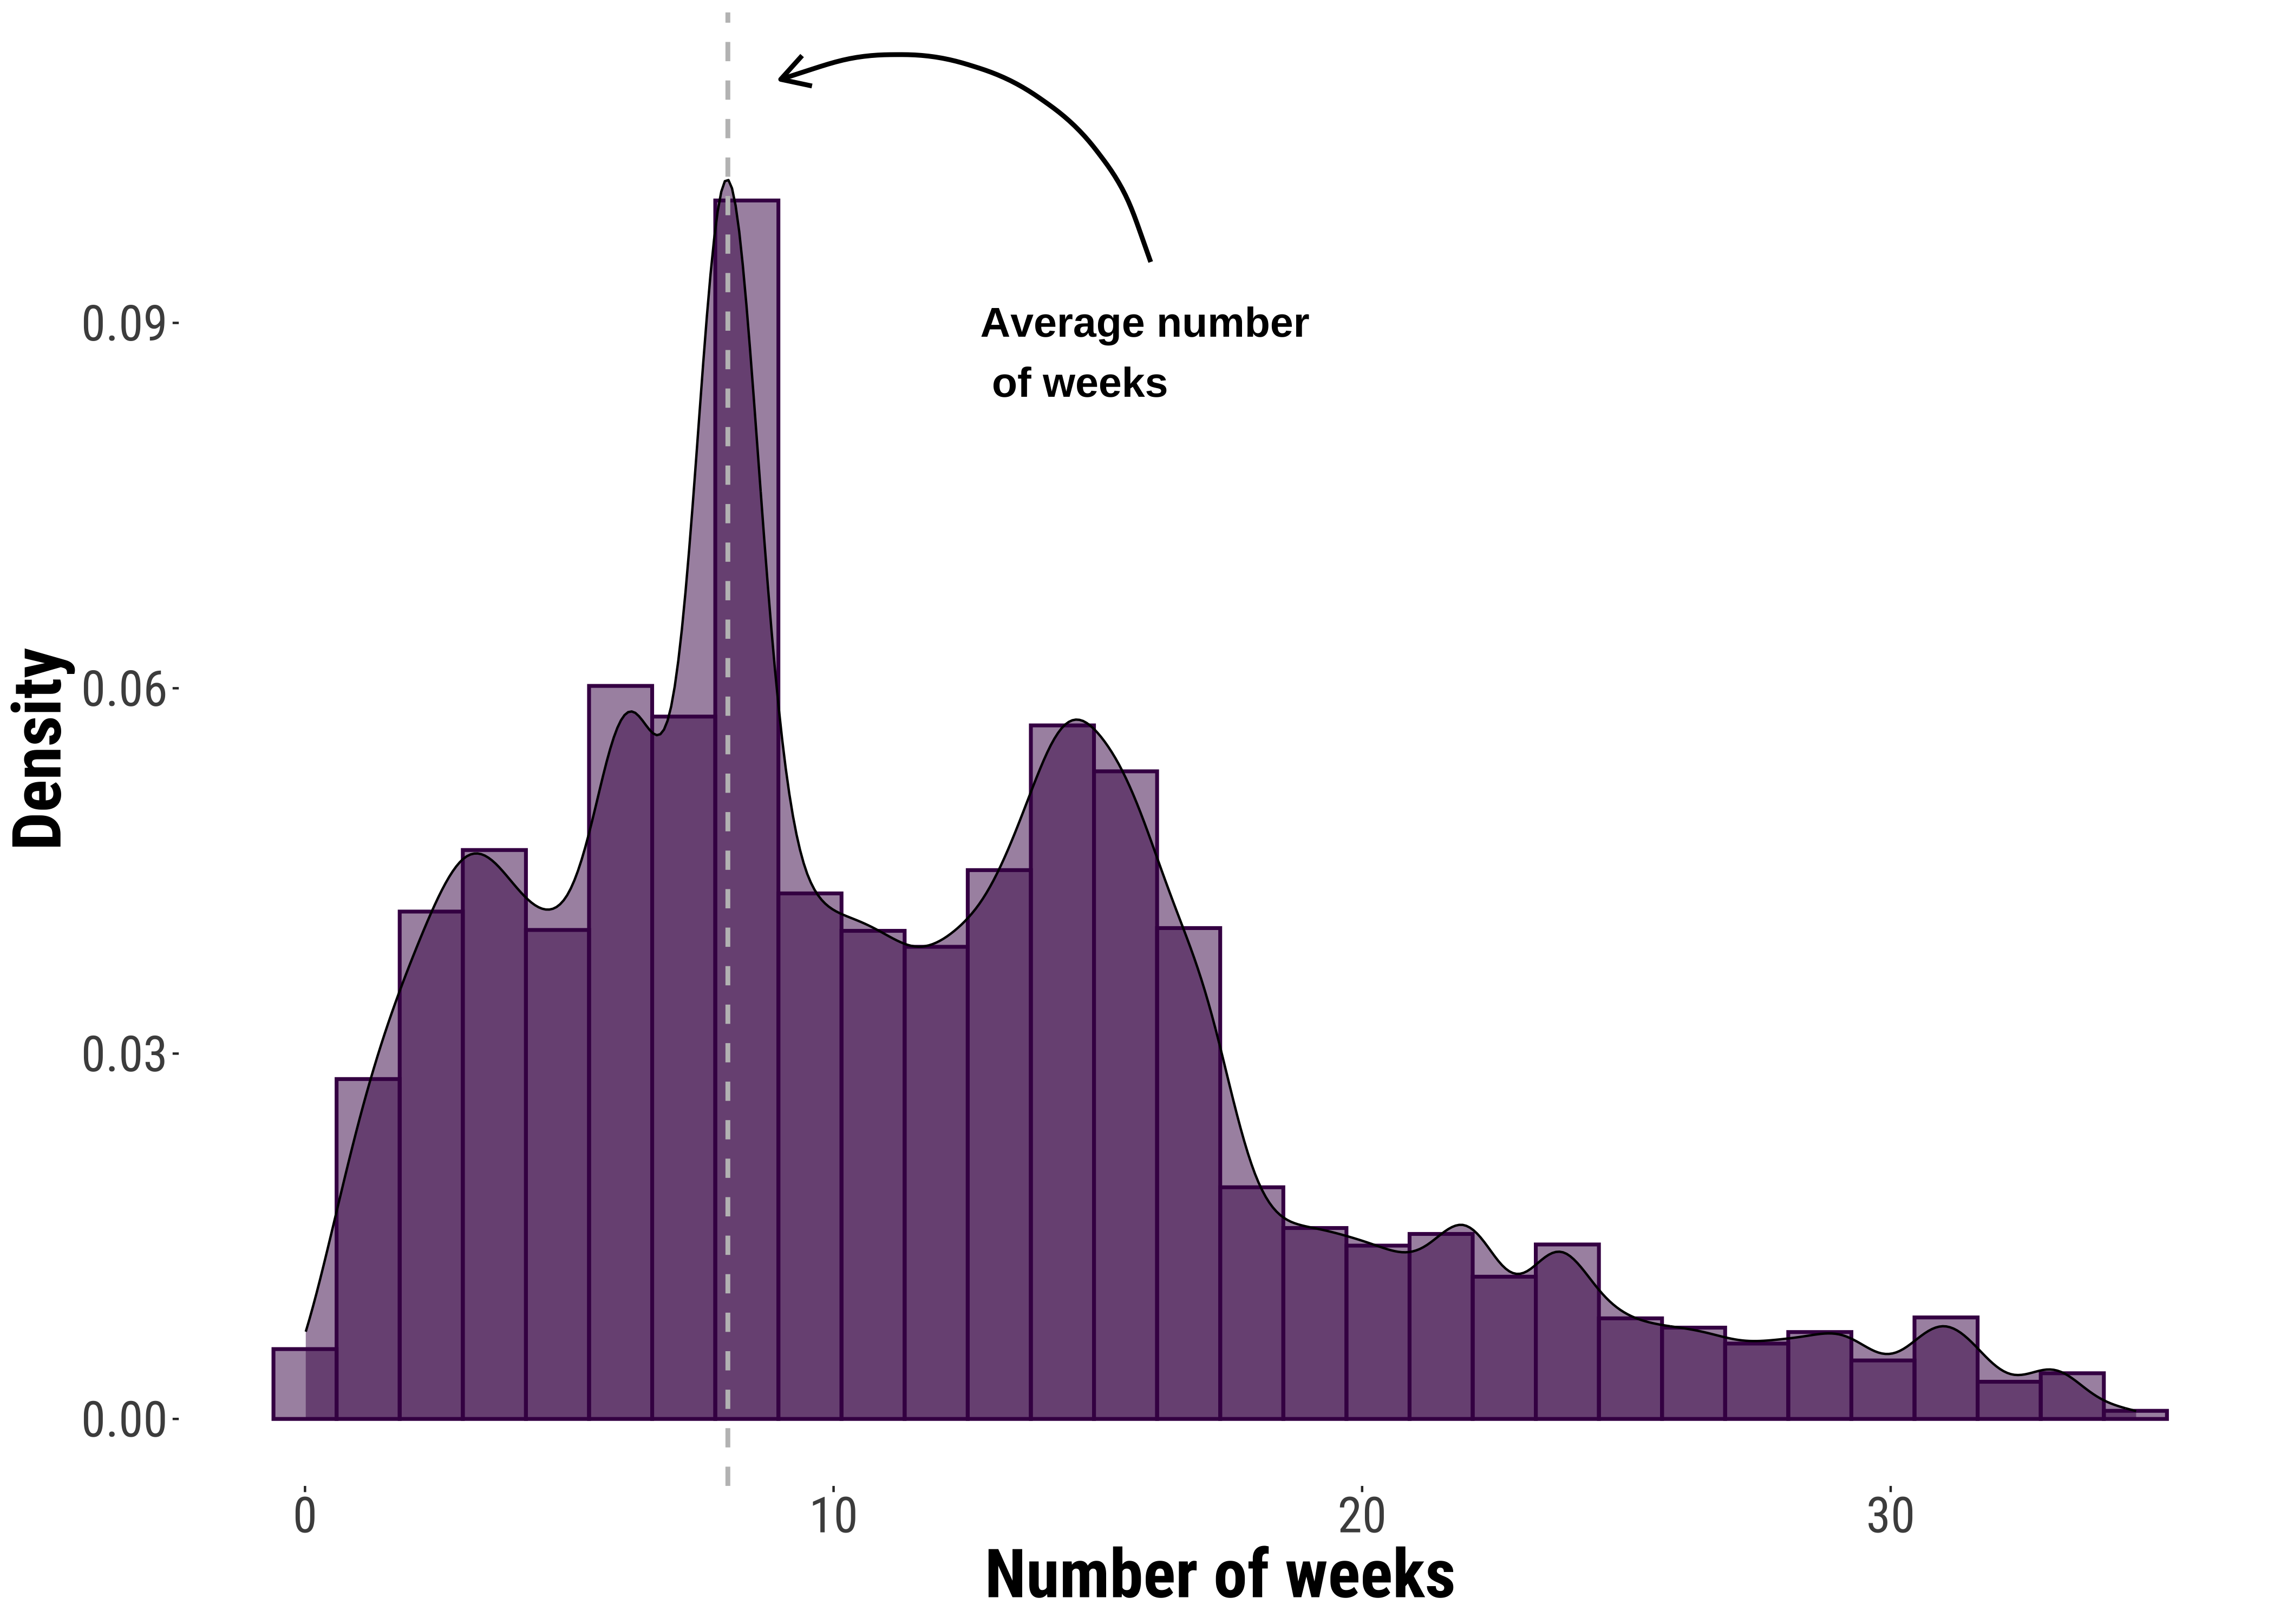
\includegraphics[width=5.20833in,height=\textheight,keepaspectratio]{../outputs/sm/returns-duration.png}
\end{center}
\end{minipage}%

\end{figure}%




\end{document}
